\documentclass{article}
\usepackage{tikz}
\usepackage{amsmath}
\usepackage{bm}
\usepackage{scalerel}
\usepackage{pgfplots}
\usepackage{mathpazo}
\pgfplotsset{width=9cm,compat=1.8}
\usetikzlibrary{patterns}
\usetikzlibrary{arrows,shapes,calc}
\usetikzlibrary{external}
\tikzset{external/system call={pdflatex \tikzexternalcheckshellescape -halt-on-error
        -interaction=batchmode -jobname "\image" "\texsource" && %  or ;
pdftops -eps "\image".pdf}}
\tikzexternalize




\begin{document}
	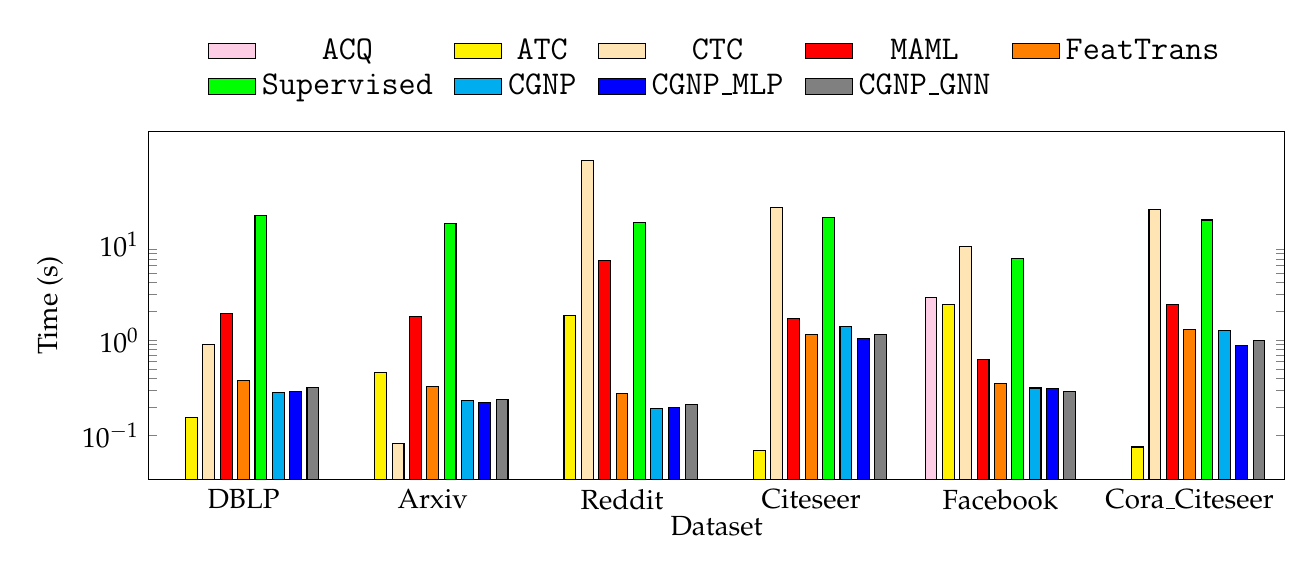
\begin{tikzpicture}
		\definecolor{lssfre}{HTML}{fccde5} %粉
		\definecolor{lssemb}{HTML}{bc80bd} %紫色
		\definecolor{lsscon}{HTML}{bebada} %淡紫色
		\definecolor{wj}{HTML}{fb8072} %橙色 深一点
		\definecolor{impr}{HTML}{80b1d3} %青蓝
		\definecolor{cs}{HTML}{fdb462} %橙色
		\definecolor{cset}{HTML}{b3de69}%绿色
		\definecolor{jsub}{HTML}{8dd3c7} %青绿
		\definecolor{sumrdf}{HTML}{ffffb3} %淡黄
		\definecolor{bsk}{HTML}{d9d9d9} %浅灰
		\definecolor{gflow}{HTML}{778899} %深灰色
		\definecolor{SB}{HTML}{F5F5DC}
		\definecolor{lc}{HTML}{FFFDD0}
		\definecolor{fire}{HTML}{FFE5B4}
		\definecolor{bo}{HTML}{E6E6FA}
		\definecolor{ye}{HTML}{FFCC00}
		\centering
		\begin{axis}
			%\label{fig:train time}
			[
			ybar, %axis on top,
			height=6cm, 
			width=16cm,
			bar width=0.15cm,
			tick align=inside,
			%enlarge y limits={value=.1,upper},
			%ymin=0, ymax=100000,
			tickwidth=0pt,
			ymode=log,
			log origin=infty,
			enlarge x limits=true,
			legend style={
				draw=none,
				at={(0.5, 1.3)},
				anchor=north,
				legend columns=5,
				/tikz/every even column/.append style={column sep=0.2cm}
			},
			ylabel={Time (s)},
			ytick={0.1, 1, 10},
			%yticklabels={$1$,$10^2$, $10^4$},
			xmin=3, xmax = 18,
			xtick={3,6,9,12,15,18 },
			xticklabels={DBLP, Arxiv, Reddit, Citeseer, Facebook, Cora\_Citeseer},
			xlabel={Dataset},
			xlabel style={yshift=1ex},
			%symbolic x coords={
			%	Arxiv, Citeseer, Cora, Facebook, Cora\_Citeseer },
			%xtick=data,
			]
			
			%ACQ
			\addplot [ybar, fill=lssfre, area legend] coordinates {
				(15,2.76)
			};
			
			%ATC
			\addplot [ybar, fill=yellow, area legend] coordinates {
				(3, 0.155)
				(6, 0.454)
				(9, 1.793)
				(12, 0.07)	
				(15,2.354)
				(18,0.076)
			};
			
			%CTC
			\addplot [ybar, fill=fire, area legend] coordinates {
				(3,0.897)
				(6,0.082)
				(9,75.75)
				(12,24.5807)
				(15,9.4582)
				(18,23.309)
			};
			
			% MAML
			\addplot [ybar, fill=red, area legend] coordinates {
				(3, 1.8917)
				(6, 1.7802)
				(9, 6.856)
				(12, 1.6912)	
				(15, 0.6296)	
				(18, 2.3752)
			};
			
			% FeatTrans
			\addplot [ybar, fill=orange, area legend] coordinates {
				(3,0.3758)
				(6,0.3246)
				(9,0.2769)
				(12,1.1528)	
				(15,0.3521)
				(18,1.2963)
			};
			
			%supervise
			\addplot [ybar, fill=green, area legend] coordinates {
				(3, 20.1437)
				(6, 16.4734)
				(9, 17.1498)
				(12,19.1957)	
				(15,7.2001)
				(18,18.0642)
			};
			
			% CGNP
			\addplot [ybar,fill=cyan, area legend] coordinates {	
				(3, 0.2837)
				(6, 0.235)
				(9, 0.1936)
				(12, 1.3911)	
				(15,0.3153)
				(18,1.2543)
			};
			
			% CGNP_MLP
			\addplot [ybar, fill=blue, area legend] coordinates {
				(3, 0.2868)
				(6, 0.2241)
				(9, 0.1959)
				(12, 1.0279)	
				(15, 0.3137)
				(18,0.8717)
			};
			
			% CGNP_GNN
			\addplot [ybar, fill=gray, area legend] coordinates {
				(3,0.318)
				(6,0.2369)
				(9,0.2098)
				(12,1.1393)	
				(15,0.2906)
				(18,0.9863)
			};
			

			
			\legend{
			    \large $\texttt{ACQ}$,
			   	\large $\texttt{ATC}$,
			   	\large $\texttt{CTC}$,
			    \large $\texttt{MAML}$,
				\large $\texttt{FeatTrans}$,
				\large $\texttt{Supervised}$,
				\large $\texttt{CGNP}$,
				\large $\texttt{CGNP\_MLP}$,
				\large $\texttt{CGNP\_GNN}$
			}
			
		\end{axis}
	\end{tikzpicture}

\end{document}
